\subsection{Modelo básico de optimización de precio}
Partiendo de la información proporcionada en \cite{Talluri2019}, se la optimización de precio es un problema en el cual se busca maximizar las ganancias de la empresa. Estas ganancias están establecidas por la Ecuación \ref{eq:revenue}, donde $p$ representa el precio de un producto individual, $D(p)$ representa la función de demanda del producto al precio $p$, y $R(p)$ representan las ganancias al precio $p$.

\begin{equation}\label{eq:revenue}
	R(p)=pD(p)
\end{equation}

La función de demanda suele asumirse de forma natural que suele disminuir su valor conforme el precio incrementa, por ello es fácil representar dicha función como una función lineal. Esta función se presentan en la Ecuación \ref{eq:demand}, donde $a$ y $b$ son los parámetros de nuestro modelo que son estimado tras observaciones previas de la variación del precio y la demanda.

\begin{equation}\label{eq:demand}
	D(p)=a-bp
\end{equation}

Implementando la sustitución pertinente, tenemos que el modelo básico optimización de precio consiste en encontrar el $p$ que maximiza el valor de $R(p)$, el cuál está descrito por la Ecuación \ref{eq:price}.

\begin{equation}\label{eq:price}
	R(p)=p(a-bp)
\end{equation}


\subsection{Selección poligámica aleatoria}
En la selección poligámica aleatoria se forma parejas de forma aleatoria, sin importar si algún individuo es emparejado más de 1 vez. Una desventaja de este método es que existe la posibilidad de no seleccionar a un individuo, lo cuál podría ocasionar que no se explore completamente el espacio de búsqueda. En la Figura \ref{fig: selection_poli} podemos observar una representación gráfica de este mecanismo de selección.


\subsection{Cruza de dos puntos}
La cruza de dos puntos (two point crossover, en inglés) es un método de recombinación comúnmente utilizado en algoritmos genéticos que permite la combinación de características de dos padres para generar una descendencia. Este método permite generar combinaciones de características de ambos padres para explorar y buscar mejores soluciones. En terminos generales, este método consta de los siguientes pasos:

\begin{enumerate}
	\item Definición de Puntos de Corte: Se seleccionan dos puntos de corte en la representación de los padres. Estos puntos dividen a los padres en tres segmentos: el segmento antes del primer punto de corte, el segmento entre los dos puntos de corte y el segmento después del segundo punto de corte.
	\item Creación de Descendencia: La descendencia se crea intercambiando los segmentos intermedios (el segmento entre los dos puntos de corte) de los dos padres. El resultado es un nuevo individuo que combina partes de ambos padres.
\end{enumerate}

\begin{figure}[htbp]
	\centering
	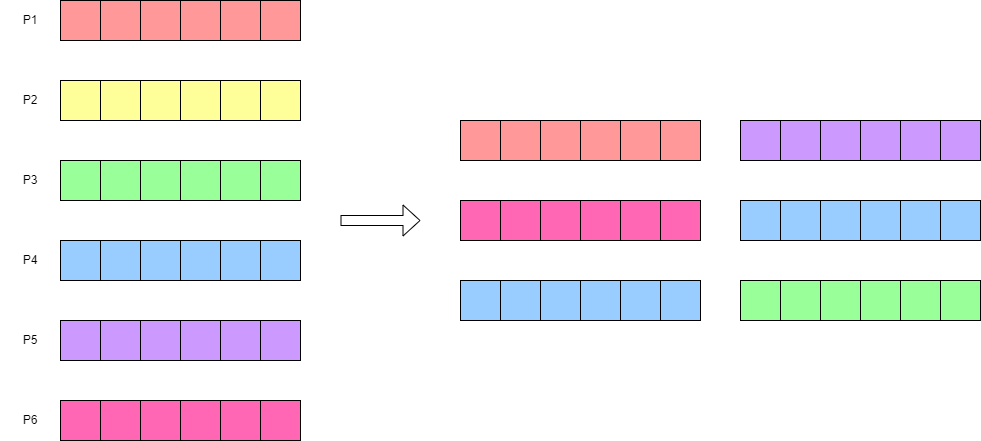
\includegraphics[width=0.8\textwidth]{random_poligamica}
	\caption{Mecanismo de selección poligámica aleatoria.}
	\label{fig: selection_poli}
\end{figure}


\begin{figure}[htbp]
	\centering
	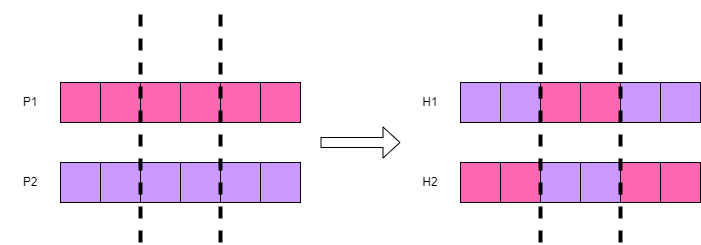
\includegraphics[width=0.8\textwidth]{crossover_two}
	\caption{Mecanismo de cruza de dos puntos.}
	\label{fig: cross_two}
\end{figure}

\newpage
\subsection{Mutación por inversión}
La mutación por inversión, o ``Inverse Mutation", es otra técnica de mutación usada en algoritmos genéticos que trabajan con soluciones representadas como permutaciones. El procedimiento de esta técnica consta de los siguientes pasos:

\begin{enumerate}
	\item Selección de segmento: Se seleccionan aleatoriamente dos puntos en la permutación. Estos puntos determinarán el inicio y el fin de un segmento.
	\item Inversión: El segmento delimitado por estos dos puntos se invierte, es decir, el orden de los alelos dentro de este segmento se revierte.
\end{enumerate}

Este mecanismo se puede observar en la Figura \ref{fig:InvM}.

\begin{figure}[htbp]
	\centering
	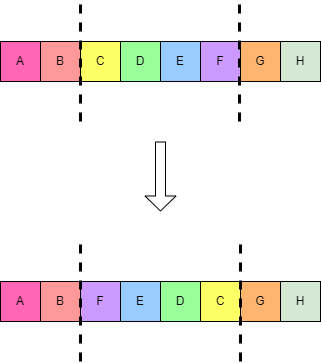
\includegraphics[width=0.3\textwidth]{inverse_mutation}
	\caption{Diagrama de funcionamiento de inverse mutation.}
	\label{fig:InvM}
\end{figure}


\subsection{Competencia genética}
El concepto de competencia genética se asemeja a la lucha por la supervivencia en la naturaleza, donde los individuos más aptos tienen una mayor probabilidad de sobrevivir y reproducirse, transmitiendo así sus genes a la siguiente generación. La idea principal detrás de la competencia genética en algoritmos evolutivos es simular este proceso de selección natural para buscar soluciones óptimas o mejores en un espacio de búsqueda.

En este proceso se toma a todos los padres y a todos los hijos, se ordenan de mayor a menor aptitud, y solamente se permitirá que pasen a la siguiente generación aquellos que presentan mejor aptitud, sin importar sin son padres o hijos.
